%!TEX root = ../main.tex
\subsection{Objectives} % (fold)
\label{sub:objectives}
	The objective of this project is to create a credit card recommender system that will recommend the most suitable credit card (from major banks in Singapore) to a consumer based on their spending habits and preferences. The system will make use of \textbf{rule-based reasoning} and \textbf{fuzzy logic}, to match the consumer’s input against a database of credit card features. As the system features most of the major banks in Singapore, it should be applicable to almost anyone living in Singapore.

	The primary target audience of our system are consumers, people from the general public. However, our system can also very much be utilised by banks as a tool for market awareness, evaluation, as well as training.

	By inputting in their preferences and spending habits, our system will be able to analyse and reason based on the inputs, and finally recommend a credit card that is most beneficial to them. Banks can also make use of our system to understand the competition, as well as use it to provide training and reference especially for frontline staff.
% subsection objectives (end)

\subsection{Success Measurements} % (fold)
\label{sub:success_measurements}

	\subsubsection{Knowledge Model} % (fold)
	\label{ssub:knowledge_model}
		Knowledge modeling can be classified into three parts \cite{schreiber2001knowledge}
		\begin{enumerate}[label=(\roman*)]
			\item Knowledge identification
			\item Knowledge specification
			\item Knowledge refinement
		\end{enumerate}
		Different tasks and components are done at each stage to derive the final recommendation of ideal credit card.
	% subsubsection knowledge_model (end)

	\subsubsection{Knowledge Identification} % (fold)
	\label{ssub:knowledge_identification}
		Knowledge identification sets the groundwork for the next stage encompassing knowledge specification. Information sources that are deemed to be useful are identified in preparation of knowledge acquisition. In the context of building a recommender system for credit card recommendation, three main sources have been identified and are documented in Table \ref{table:knowledgesource}.

		\begin{table}[h]
		\centering
		\resizebox{\textwidth}{!}{%
		\begin{tabular}{|l|p{3cm}|p{7cm}|p{5cm}|}
		\hline
		\textbf{S/N} & \textbf{Source of Information} & \textbf{Insights from information sources}                                                                                                                                                 & \textbf{Knowledge acquisition technique}                                                        \\ \hline
		\textbf{1}   & Credit card websites           & It provides basic information on credit card requirements and credit card benefit.                                                                                                          & Data gathering from publicly available/documented information.                                  \\ \hline
		\textbf{2}   & Banker Expert                  & The subject matter expert, will be able to:Identify and explain the considerations in choosing a credit card. Validate or further reinforce our understanding from the credit card website & Elicitation of tacit knowledge through the conduct of interview                                 \\ \hline
		\textbf{3}   & Generic Population             & To validate and support the claims from the business expert with data.To validate and finalize features selection with data.                                                               & Elicitation of tacit knowledge through analysis results of a survey from the general population \\ \hline
		\end{tabular}%
		}
		\caption{Knowledge Source and Acquisition Technique}
		\label{table:knowledgesource}
		\end{table}
	% subsubsection knowledge_identification (end)

	\subsubsection{Knowledge Acquisition} % (fold)
	\label{ssub:knowledge_acquisition}
		Following from the identification of knowledge sources, knowledge acquisition is conducted to capture the problem-solving domain knowledge. The techniques adopted to acquire the knowledge have been describe in Table \ref{table:knowledgesource} and the corresponding results are presented using a dependency diagram as shown in Figure \ref{fig:knowledge_model}.

		\begin{figure}[h]
			\centering
			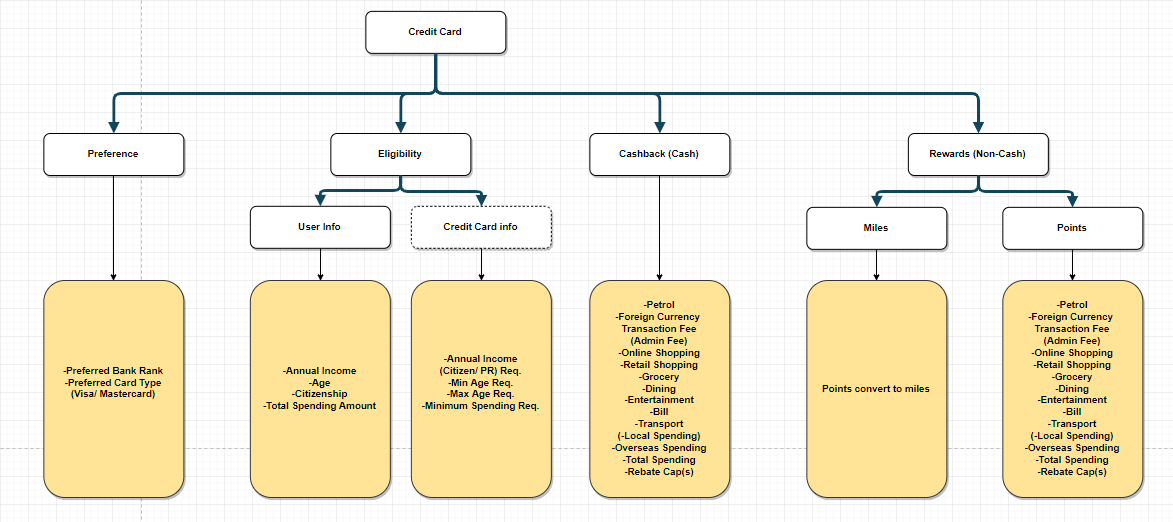
\includegraphics[width=\linewidth]{img/knowledge_model.png}
			\caption{Dependency Diagram of Credit Card Recommendation System}
			\label{fig:knowledge_model}
		\end{figure}

		The dependency diagram arranges the factors affecting applicant’s choice of credit cards in a hierarchical tree structure. The top most level node represents the description of the proposed system, which in this case, recommends a group of credit cards to the user. This decision can be broken down into multiple layers of inferable sub-goals or sub-factors before arriving at a list of “observables”. These “observables” are gathered from users of the proposed system and they represent their inherent preference. Table \ref{table:exampe_depedency} illustrates an example using the dependency diagram in Figure \ref{fig:system_architecture_diagram}.

		The inferable sub-goals together with the “observables” are in fact, derived from the advices and insights provided by the domain expert and following validated by survey results. Full interview transcript and audio, together with the survey results and analysis, are appended in \textit{Appendix C} for submission.

		\begin{table}[]
		\centering
		\resizebox{\textwidth}{!}{%
		\begin{tabular}{|l|p{4cm}|p{9cm}|}
		\hline
		\textbf{S/N} & \textbf{Category}   & \textbf{Information}                                                                                  \\ \hline
		\textbf{1}   & Observable          & A client who spends a lot on dining.                                                                  \\ \hline
		\textbf{2}   & Inferable Sub-goals & The client in {[}1{]} might be interested in a credit card with Cashback or Reward points for dining. \\ \hline
		\textbf{3}   & Top-level inference & The sub-goal in {[}2{]} is also one of the main factors that a client choose a suitable credit card.  \\ \hline
		\end{tabular}%
		}
		\caption{Example to Show A Part of the Dependency Diagram}
		\label{table:exampe_depedency}
		\end{table}
	% subsubsection knowledge_acquisition (end)

	\subsubsection{Knowledge Specification} % (fold)
	\label{ssub:knowledge_specification}
		After data is acquired from Banks Credit Card website, the next stage is to transform the unstructured data into decision-making domain knowledge, and this would require to form a calculation logic for different types of credit card.

		Data from the Credit Card Website only mentions the maximum cashback/reward that a client can get, while the terms and conditions specify the criteria and cap for each spending category. Our team did an analysis and establish the formula to calculate cash back or reward points:

		\lstset{basicstyle=\footnotesize\ttfamily}
		% \lstset{frame=bottomline}
		\begin{lstlisting}[frame=single, gobble=11, tabsize=4, showstringspaces=false, mathescape]
			Cashback of Credit Card =

			IF Minimum Spending is met, THEN
			$\sum$(min(Credit Card Spending each category * Cash Back Higher Rate,
					Cap of cashback of the category))
			ElSE
			$\sum$(min(Credit Card Spending each category * Cash Back Lower Rate,
					Cap of cashback of the category))
			END

			Reward Points of Credit Card = $\sum$(Round_Down_To_Nearest_Integer
			(Credit card each category spending amount/Reward Point Lot)*
			Reward Point Multiplier)

			Miles of Credit Card = Reward Points of Credit Card *
			Reward Point to Miles conversion rate
		\end{lstlisting}

		Based on User’s spending / estimated spending amount on each category, the logic can calculate the maximum Cashback/Reward Points for each credit card, compare and recommend the most suitable one for consumer.

		User’s preference would determine which type of credit card the system recommends. If user only choose Cashback Card, the system will only take Cashback card into consideration. If user are open to both Cashback and Reward card, the system will convert the reward points to an equivalent cash value and suggest the most valuable (maximum cashback) card to user.

		The conversion between Reward Points to Cashback Value is done via Fuzzy logic.

		\begin{lstlisting}[frame=single, gobble=11, tabsize=4, showstringspaces=false, mathescape]
			Cash Value = Reward Points / Fuzzy Factor
		\end{lstlisting}

	% subsubsection knowledge_specification (end)

	\subsubsection{Knowledge Refinement} % (fold)
	\label{ssub:knowledge_refinement}
		The Knowledge Refinement would be an iterative process and it includes model validation and model refinement. For model validation, different sets of test data will be used to run simulation, and the result will be compared with current spending habit data.

		For model refinement, certainty factors is included to incorporate the uncertainty of user preference and change of terms and conditions of the card. The model needs to be revised periodically with live data.

	% subsubsection knowledge_refinement (end)

% subsection success_measurements (end)